\section[Die soziale Frage nach \Nam{}{Hegel}]
{Die soziale Frage nach \Nam{}{Hegel}\mycite{HegelGrundl}}
\label{sec:soz-frag-heg}
\index{Soziale Fragel!nach Hegel}
\Nam{Hegel, Georg Wilhelm Friedrich}{}

Zur Problematik der sozialen Frage nach \Nam{}{Hegel} siehe die Abbildungen
\ref{pic:soz-frag-sch} und \ref{pic:soz-frag-sch-rev}.

\begin{figure}
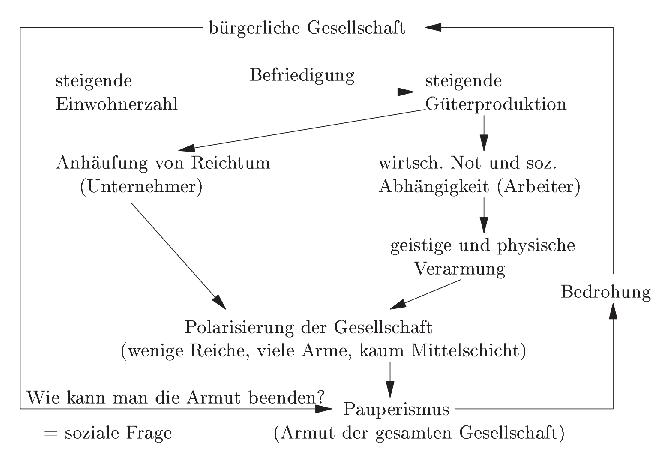
\includegraphics[width=\textwidth]{soz-frag-sch.eps}
\caption{Entstehung der sozialen Frage nach \Nam{}{Hegel}}
\label{pic:soz-frag-sch}
\end{figure}

\begin{figure}
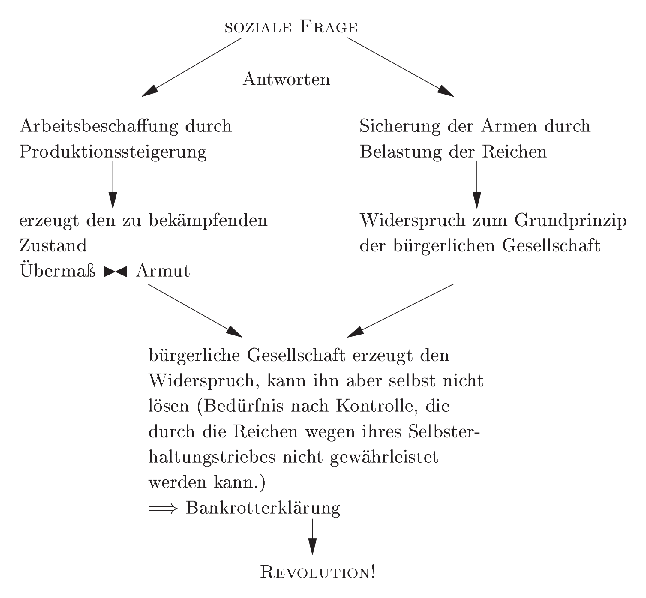
\includegraphics[width=\textwidth]{soz-frag-sch-rev.eps}
\caption{Folgen der sozialen Frage nach \Nam{}{Hegel}}
\label{pic:soz-frag-sch-rev}
\end{figure}

\endinput
